\byline{{\textbf{\Large\sffamily December Bonsai Club Meetup:}}\\
        {\textbf{\large\sffamily A Joyful and Reflective Evening}}}{The Newsletter Team}
\noindent
Our December bonsai club meeting was a fantastic way to close the year, with more than 20 members gathering to share ideas, work on trees, and celebrate the festive season.
The night featured lively discussions, practical demonstrations, and moments of reflection, making it a memorable event for all who attended.

A highlight of the evening was the \textbf{Dave}'s \textbf{Tree Critique Corner}, the new format for the tree critique established during our recent AGM.
Members brought their bonsai for constructive feedback, sparking fascinating conversations about styling, health, and long\--term development.
Meanwhile, the worktables were bustling as members refined their trees and shared opinions on \textbf{suiseki}.

We also enjoyed the return of the \textbf{Tree of the Month} competition.
This month's theme was \emph{``Christmas trees,''} with separate sections for experienced and novice members won respectively by \textbf{Tony Ulatowski}'s beautifully styled \emph{Pinus Nigra} and \textbf{Stefano Bragaglia}'s charming \emph{Ficus Benjamina}.

Amid the festivities of mince pies, drinks, and laughter, we paused to honor \textbf{Andy Pearson}, an internationally recognised potter who recently passed away unexpectedly.
His contributions to the bonsai community and his artistry will be greatly missed.

Thank you to everyone who joined us for this joyful evening.
Merry Christmas to all, and we look forward to seeing you at next month's meeting!

\begin{window}[2,l,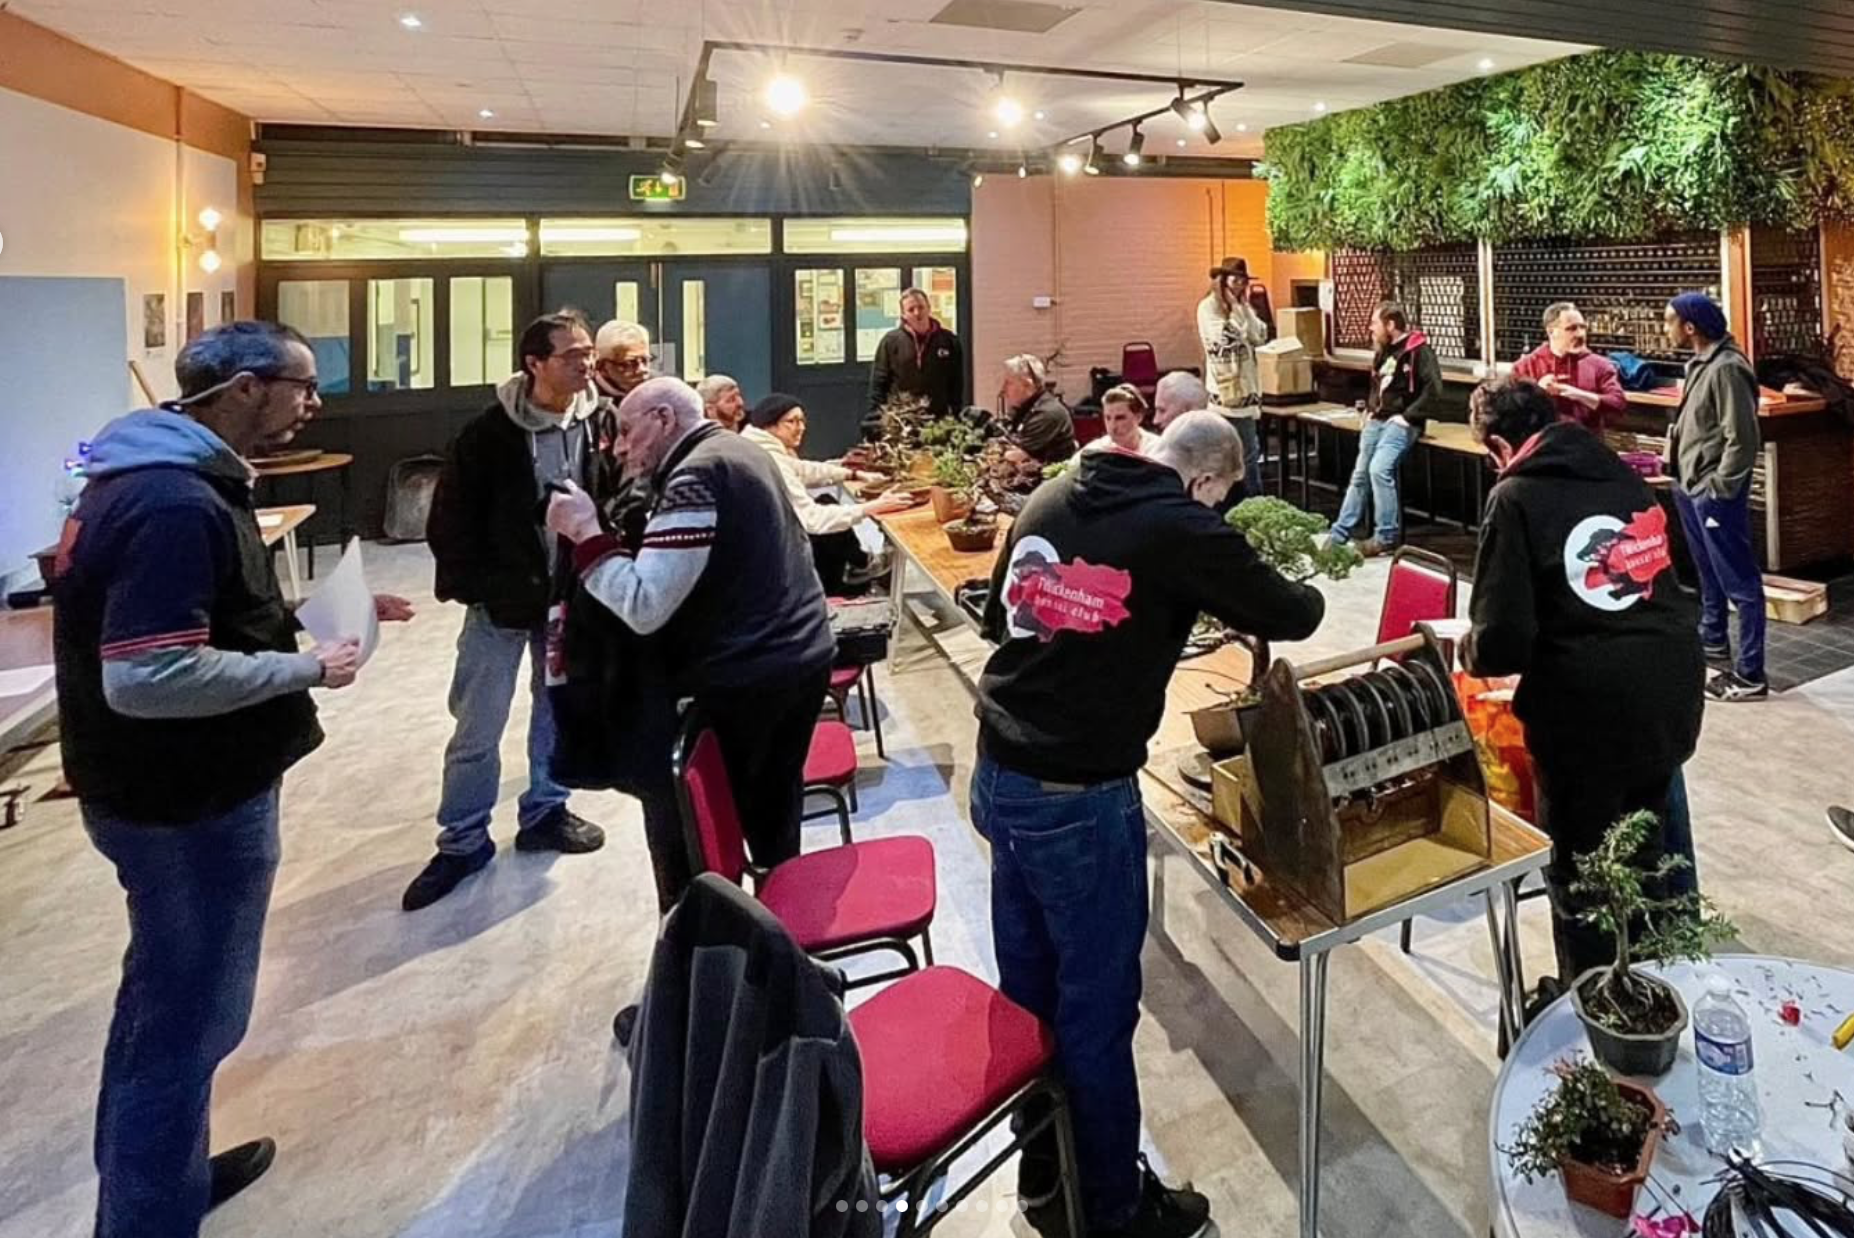
\includegraphics[width=1.0\columnwidth]{2024_12/res/editorial.png},\centerline{\emph{The Whitton Community Centre buzzes for the Bonsai Club's Dec 2024 meetup.}}]
\end{window}

\closearticle
\clearpage